\documentclass[12pt]{article}
\usepackage[left=2cm,right=2cm,top=2cm,bottom=2cm,bindingoffset=0cm]{geometry}
\usepackage[utf8x]{inputenc}
\usepackage[english,russian]{babel}
\usepackage{cmap}
\usepackage{amssymb}
\usepackage{amsmath}
\usepackage{url}
\usepackage{pifont}
\usepackage{tikz}
\usepackage{verbatim}

\usetikzlibrary{shapes,arrows}
\usetikzlibrary{positioning,automata}
\tikzset{every state/.style={minimum size=0.2cm},
initial text={}
}


\newenvironment{myauto}[1][3]
{
  \begin{center}
    \begin{tikzpicture}[> = stealth,node distance=#1cm, on grid, very thick]
}
{
    \end{tikzpicture}
  \end{center}
}


\begin{document}
\begin{center} {\LARGE Формальные языки} \end{center}

\begin{center} \Large домашнее задание до 23:59 09.03 \end{center}
\bigskip

\begin{enumerate}
  \item Построить полный минимальный детерминированный конечный автомат, распознающий язык:
  \[
    \{ \omega \in \{ a, b \}^* \mid |\omega|_a \ge 2, |\omega|_b \ge 2 \}
  \]
  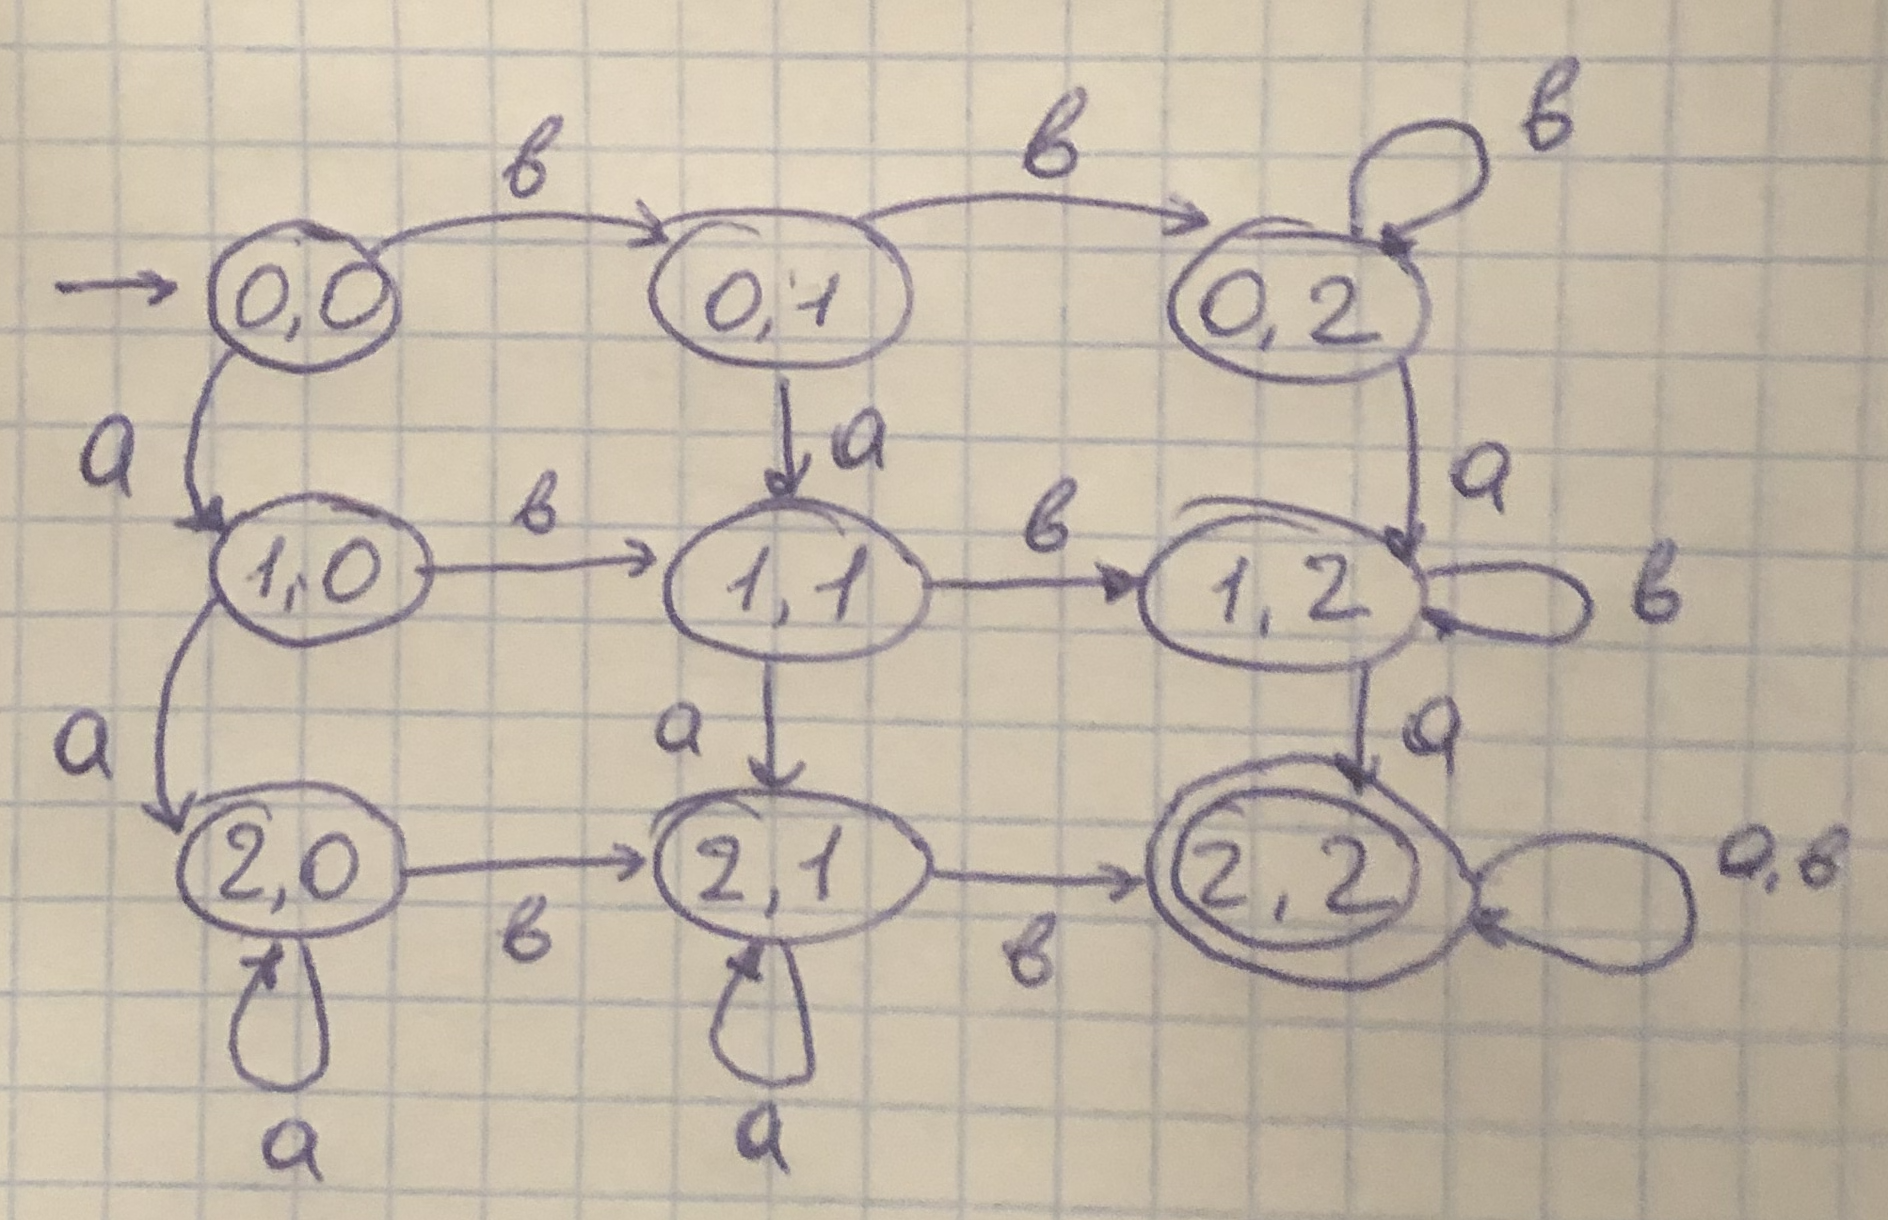
\includegraphics[width=15cm, height=6cm, keepaspectratio]{./n1.png}
  \item Построить полный минимальный ДКА, эквивалентный данному:
  \begin{myauto}
    \node[state,initial]   (q_0) {$q_0$};
    \node[state]           (q_1) [right=of q_0] {$q_1$};
    \node[state]           (q_2) [right=of q_1] {$q_3$};
    \node[state,accepting] (q_3) [right=of q_2] {$q_4$};

    \path[->] (q_0) edge [loop above] node [above] {$a, b$} ()
                    edge              node [above] {$b$}    (q_1)
              (q_1) edge              node [above] {$a, b$} (q_2)
              (q_2) edge              node [above] {$a, b$} (q_3)
    ;
  \end{myauto}
  
  \item Построить минимальный конечный автомат, распознающий язык натуральных чисел в десятичной системе без лидирующих нулей, делящихся на 4 и имеющих сумму цифр, равную 2.
  \\
  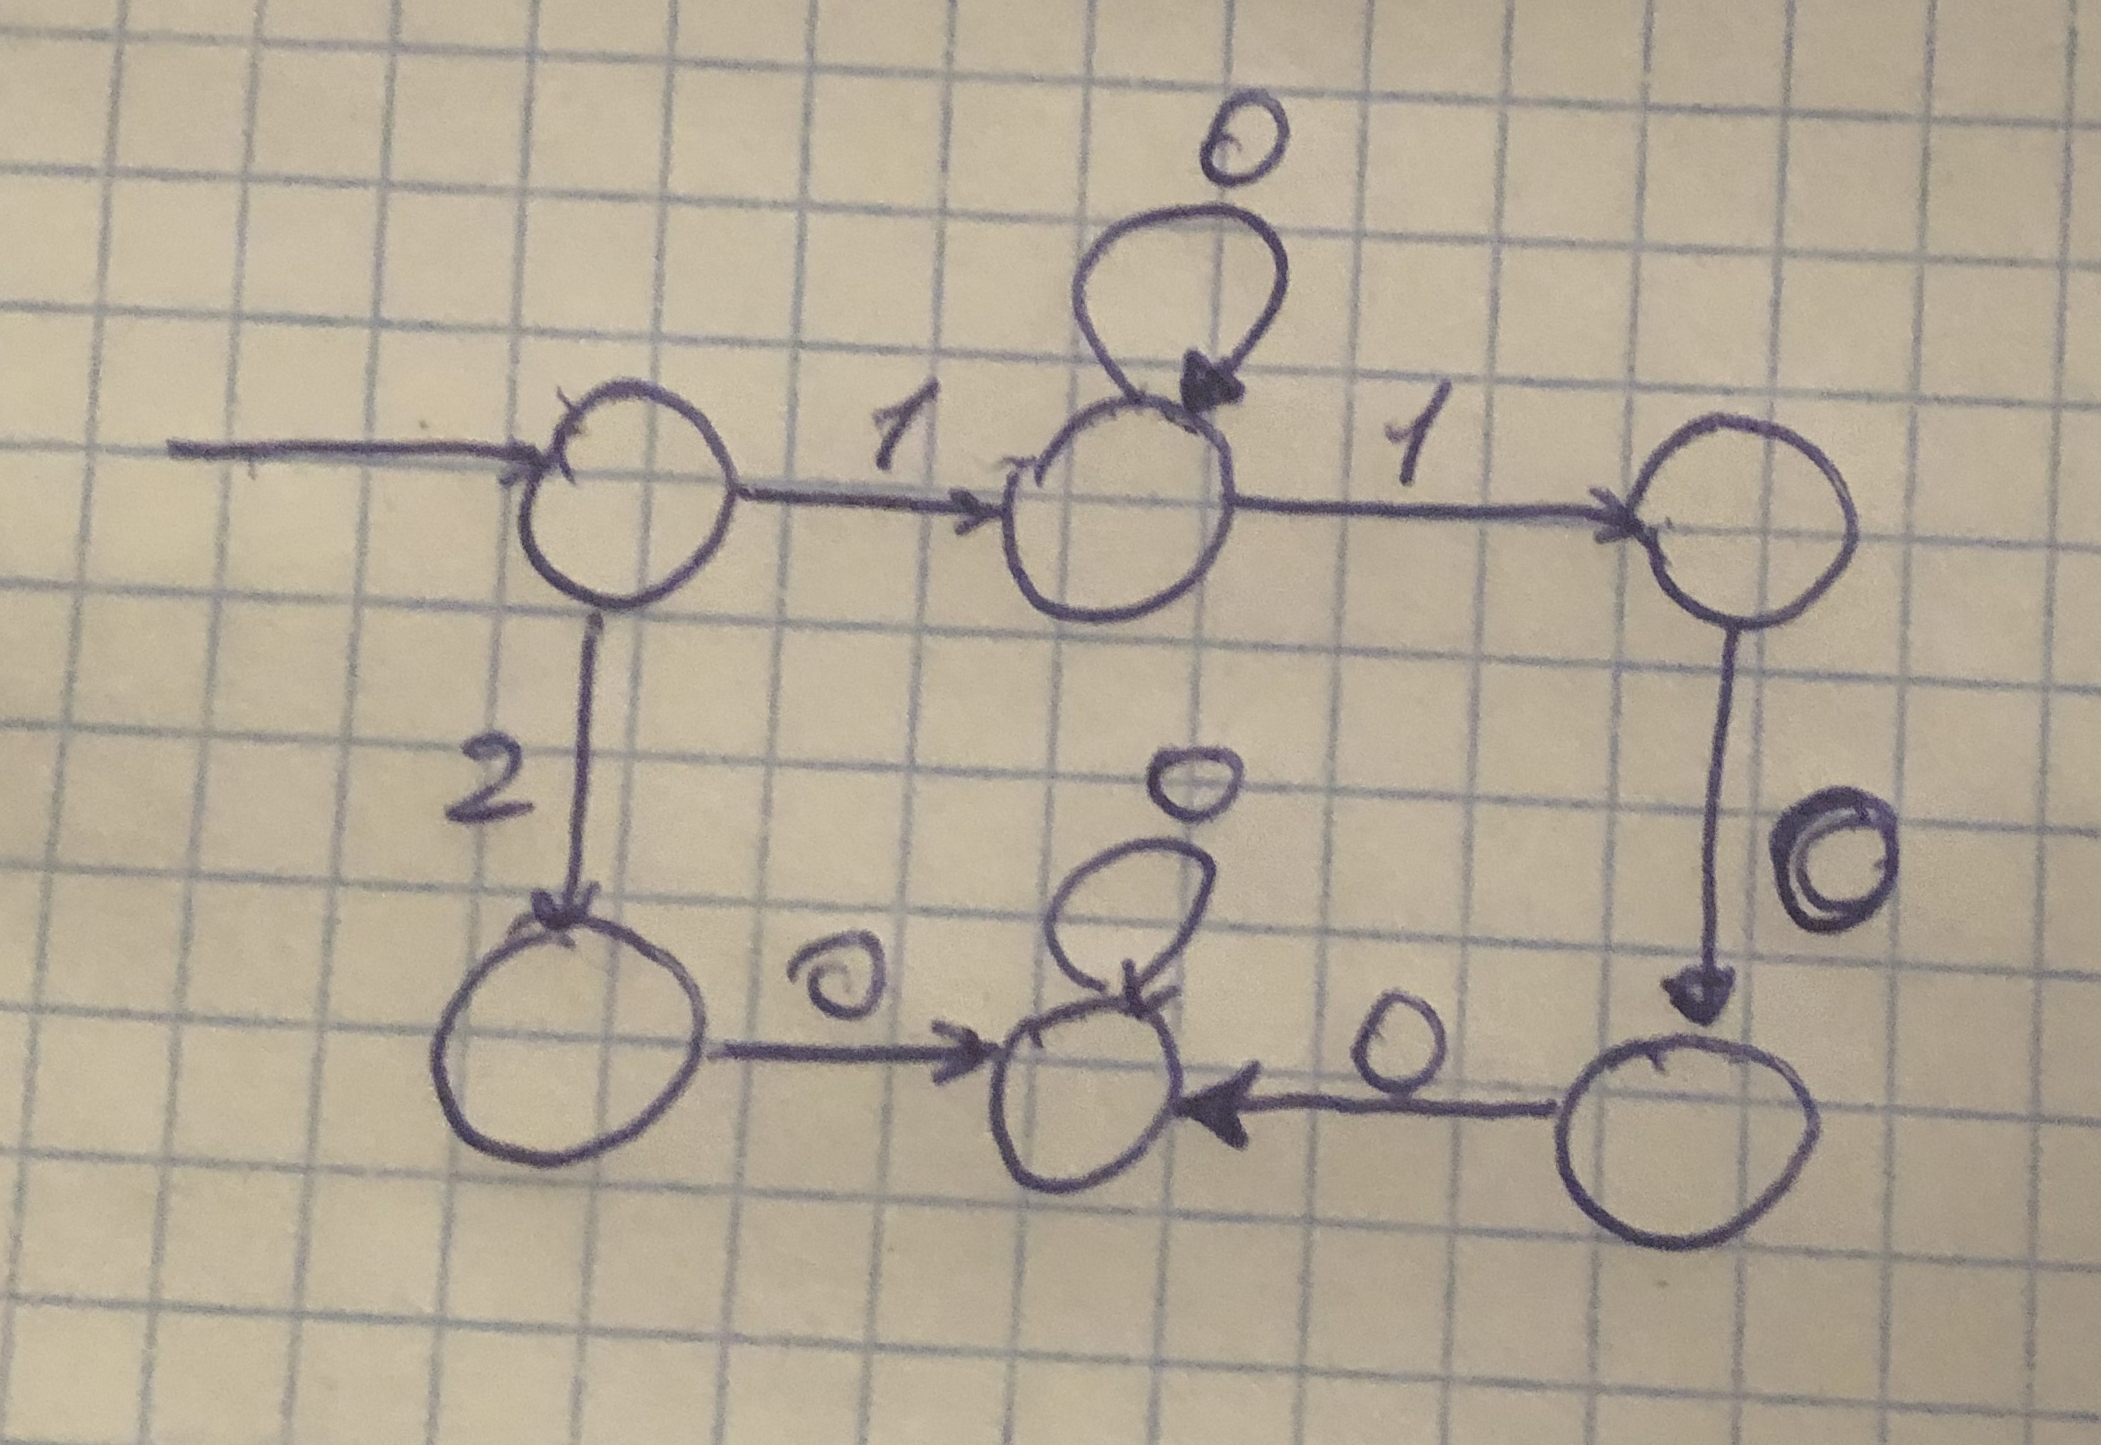
\includegraphics[width=15cm, height=6cm, keepaspectratio]{./n3.png}
\end{enumerate}

\newpage

\begin{center}
  \Large{Пример применения алгоритма минимизации}
\end{center}

\bigskip

Минимизируем данный автомат:

\begin{center}
  \begin{tikzpicture}[> = stealth,node distance=3cm, on grid]
    \node[state]           (q_2)                      {C};
    \node[state,initial]   (q_0) [above left=of q_2]  {A};
    \node[state]           (q_1) [below left=of q_2]  {B};
    \node[state]           (q_3) [right=of q_2]       {D};
    \node[state]           (q_4) [above right=of q_3] {E};
    \node[state,accepting] (q_5) [below right=of q_3] {F};
    \node[state,accepting] (q_6) [above right=of q_5] {G};

    \path[->] (q_0) edge [bend left=15]  node [right] {$1$} (q_1)
                    edge                 node [above] {$0$} (q_2)
              (q_1) edge [bend left=15]  node [left]  {$1$} (q_0)
                    edge                 node [below] {$0$} (q_2)
              (q_2) edge [bend right=15] node [below] {$1$} (q_3)
                    edge [bend left=15]  node [above] {$0$} (q_3)
              (q_3) edge                 node [below] {$1$} (q_5)
                    edge                 node [above] {$0$} (q_4)
              (q_4) edge                 node [above] {$1$} (q_6)
                    edge                 node [right] {$0$} (q_5)
              (q_5) edge [loop below]    node         {$1$} ()
                    edge [loop left]     node         {$0$} ()
              (q_6) edge                 node [below] {$1$} (q_5)
                    edge [loop right]    node         {$0$} ();
  \end{tikzpicture}
\end{center}

Автомат полный, в нем нет недостижимых вершин --- продолжаем.

Строим обратное $\delta$ отображение.

\begin{tabular}{c|c|c}
$\delta^{-1}$ & 0 & 1 \\ \hline
A & --- & B \\
B & --- & A \\
C & A B & --- \\
D & C & C \\
E & D & --- \\
F & E F & D F G \\
G & G & E
\end{tabular}

Отмечаем в таблице и добавляем в очередь пары состояний, различаемых словом $\varepsilon$: все пары, один элемент которых --- терминальное состояние, а второй --- не терминальное состояние. Для данного автомата это пары

$(A, F), (B, F), (C, F), (D, F), (E,F), (A, G), (B, G), (C, G), (D, G), (E, G)$

Дальше итерируем процесс определения неэквивалентных состояний, пока очередь не оказывается пуста.

$(A, F)$ не дает нам новых неэквивалентных пар. Для $(B, F)$ находится 2 пары: $(A, D), (A, G)$. Первая пара не отмечена в таблице --- отмечаем и добавляем в очередь. Вторая пара уже отмечена в таблице, значит, ничего делать не надо. Переходим к следующей паре из очереди. Итерируем дальше, пока очередь не опустошится.

Результирующая таблица (заполнен только треугольник, потому что остальное симметрично) и порядок добавления пар в очередь.

\begin{tabular}{c|cc|cc|cc|c}
& A & B & C & D & E & F & G \\ \hline
A &&&&&&& \\
B &&&&&&& \\ \hline
C & \checkmark & \checkmark &&&&& \\
D & \checkmark & \checkmark & \checkmark &&&& \\ \hline
E & \checkmark & \checkmark & \checkmark & \checkmark &&& \\
F & \checkmark & \checkmark & \checkmark & \checkmark & \checkmark && \\ \hline
G & \checkmark & \checkmark & \checkmark & \checkmark & \checkmark && \\
\end{tabular}

Очередь:

$
(A, F), (B, F), (C, F), (D, F), (E,F), (A, G), (B, G), (C, G), (D, G), (E, G),
$

$
(B, D), (A, D), (A, E), (B, E), (C, E), (C, D), (D, E), (A,C), (B, C))
$

В таблице выделились классы эквивалентных вершин: $\{A, B\}, \{C\}, \{D\}, \{E\}, \{F,G\}$. Остается только нарисовать результирующий автомат с вершинами-классами. Переходы добавляются тогда, когда из какого-нибудь состояния первого класса есть переход в какое-нибудь состояние второго класса. Минимизированный автомат:

\begin{center}
  \begin{tikzpicture}[> = stealth,node distance=3cm, on grid]
    \node[state,initial]   (q_01)                     {AB};
    \node[state]           (q_2)  [right=of q_01]      {C};
    \node[state]           (q_3)  [right=of q_2]       {D};
    \node[state]           (q_4)  [above right=of q_3] {E};
    \node[state,accepting] (q_56) [below right=of q_3] {FG};

    \path[->] (q_01) edge [loop above]    node [above] {$1$} ()
                     edge                 node [above] {$0$} (q_2)
              (q_2)  edge [bend right=15] node [below] {$1$} (q_3)
                     edge [bend left=15]  node [above] {$0$} (q_3)
              (q_3)  edge                 node [below] {$1$} (q_56)
                     edge                 node [above] {$0$} (q_4)
              (q_4)  edge [bend right=15] node [left]  {$1$} (q_56)
                     edge [bend left=15]  node [right] {$0$} (q_56)
              (q_56) edge [loop below]    node         {$1$} ()
                     edge [loop left]     node         {$0$} ();
  \end{tikzpicture}
\end{center}

\end{document}
